\documentclass[conference]{IEEEtran}

% packages
\usepackage{graphicx}   % for images
\newcommand{\MATLAB}{\textsc{Matlab}\xspace}
\usepackage{mathtools}  % obvious for equations
\usepackage{amsmath}
\usepackage{amssymb}
\usepackage[justification=centering]{caption}
\usepackage{todonotes}
\usepackage[utf8]{inputenc}
\usepackage[T1]{fontenc}
\usepackage{textcomp} % for degree
\usepackage{gensymb}

% matlab
\usepackage{listings}
\usepackage{color} %red, green, blue, yellow, cyan, magenta, black, white
\definecolor{mygreen}{RGB}{28,172,0} % color values Red, Green, Blue
\definecolor{mylilas}{RGB}{170,55,241}

\lstset{language=Matlab,%
    %basicstyle=\color{red},
    breaklines=true,%
    morekeywords={matlab2tikz},
    keywordstyle=\color{blue},%
    morekeywords=[2]{1}, keywordstyle=[2]{\color{black}},
    identifierstyle=\color{black},%
    stringstyle=\color{mylilas},
    commentstyle=\color{mygreen},%
    showstringspaces=false,%without this there will be a symbol in the places where there is a space
    numbers=left,%
    numberstyle={\tiny \color{black}},% size of the numbers
    numbersep=9pt, % this defines how far the numbers are from the text
    emph=[1]{for,end,break},emphstyle=[1]\color{red}, %some words to emphasise
    %emph=[2]{word1,word2}, emphstyle=[2]{style},
}

% we do not want indents unless specified
\newlength\tindent
\setlength{\tindent}{\parindent}
\setlength{\parindent}{0pt}
\renewcommand{\indent}{\hspace*{\tindent}}
\newcommand\abs[1]{\left|#1\right|}
\newcommand{\norm}[1]{\left\lVert#1\right\rVert}

% document, title and authors
\onecolumn
\begin{document}
\title{ET4147: Signal Processing for Communications\\
    \large Homework 3}
\author{
  \IEEEauthorblockN{Erik Hagenaars}
  \IEEEauthorblockA{4272404}
  \and
  \IEEEauthorblockN{Teun de Smalen}
  \IEEEauthorblockA{4321014}
}
\maketitle


\listoftodos
% content
\section{Introduction} \label{sec:introduction}
This report discusses the work done on the mini-project for the course "IN4182 - Digital Audio and Speech Processing". In the first chapter the overall system is described, followed by the method used for framing.
\section{System} \label{sec:system}
\subsection{Signal model}
Before the architecture of the system can be designed, the signal model and assumptions are made. For the signal model, Additive White Gaussian Noise (AWGN) is expected. If $Y$ is defined as the signal with AWGN, $S$ the desired source signal and $N$ the noise, the model can be expressed as shown in Eq. \ref{eq:signal_time} and Eq. \ref{eq:signal_freq}. In which the time domain and frequency domain expressions are shown.

\begin{align}
  Y_{t}[n] &= S_{t}[n] + N_{t}[n] \quad \text{(time domain)}
  \label{eq:signal_time} \\
  Y_{k}[l] &= S_{k}[l] + N_{k}[l] \quad \text{(frequency domain)}
  \label{eq:signal_freq}
\end{align}

To simplify the model more, some assumptions are made. The first assumption is that the source signal and noise are uncorrelated (Eq. \ref{eq:signal_uncorrelated1}). This allows for the autocorrelation of the received signal to be simplified. Since the source and noise are uncorrelated, the autocorrelation of the received signal can be expressed by the addition of the autocorrelation of the signal and the noise (Eq. \ref{eq:signal_uncorrelated2}). The second assumption is that the speech signal is wide-sense stationary (WSS) in small frames (Eq. \ref{eq:signal_wss}). Since a speech signal can be seen as a periodic signal or noise, this assumption holds in theory. In practice, speech is not stationary but the performance of the enhancement system is sufficient.

\begin{align}
  R_{S_{t}N_{t}}(n,m) &= 0 \quad \text{(uncorrelated)}
  \label{eq:signal_uncorrelated1} \\
  R_{Y_{t}Y_{t}}(n,m) &= R_{S_{t}S_{t}}(n,m) - R_{N_{t}N_{t}}(n,m)
  \label{eq:signal_uncorrelated2} \\
  R_{Y_{t}Y_{t}}(n,m) &= R_{Y_{t}Y_{t}}(m-n) \quad \text{(wide-sense stationary)}
  \label{eq:signal_wss}
\end{align}

An important property of audio is the power spectrum density (PSD). The PSD is defined as the Fourier Transform (FT) of the autocorrelation (Eq. \ref{eq:pyyk1}). And with the assumption of uncorrelated noise and source, this can be expressed as the PSD of the signal and noise added as in Eq. \ref{eq:pyyk2}. Since the frames are of finite length, an estimation of the PSD needs to be made. The estimation of Eq. \ref{eq:pyyest} is called the periodogram of the signal. To enhance this estimation, Bartlett's method can be used shown in Eq. \ref{eq:pyyBest}.

\begin{align}
  P_{YY,k} &= \lim_{L \to \infty} \sum_{m=-L/2}^{L/2} R_{Y_{t}Y_{t}}(m) e^{-j2\pi \frac{km}{K}}
  \label{eq:pyyk1} \\
  &= P_{SS,k} + P_{NN,k}
  \label{eq:pyyk2} \\
  \hat P_{YY,k}^{P}(l) &= \frac{1}{L}\abs{Y_{k}(l)}^{2}
  \label{eq:pyyest} \\
  \hat P_{YY,k}^{B}(l) &= \frac{1}{M}\sum_{m=l-M+1}^{l} \hat P_{YY,k}^{P}(m)
  \label{eq:pyyBest}
\end{align}

\subsection{System overview}
From the signal model, a few components of the system can be derived. Firstly, to hold the WSS assumption, the signal sequence needs to be split in multiple segments. This process will be expressed as Framing.
Since the PSD is an important property of the signal, it need to be converted to the frequency domain. A problem is that the FT can cause problems in the sidelobes of the frames due to Gibb's phenomenon. To avoid this, the framing function needs to window this signal frame to suppress the edges of the frame. The frames will become overlapping.
At the end of the system, the time domain representation of the signal will be recovered using the inverse FT and the frames will be merged using the overlap add method where a deframing window is used.
To estimate the source, some other properties need to be estimated from the received signal. These important properties include the estimated noise PSD, the estimated source PSD (by estimating the SNR) and if the source is present. With these properties, a gain filter can be created for the received signal which should suppress the noise and interference.
The resulting system design is shown in Fig. \ref{fig:system}.

\begin{figure}[h]
  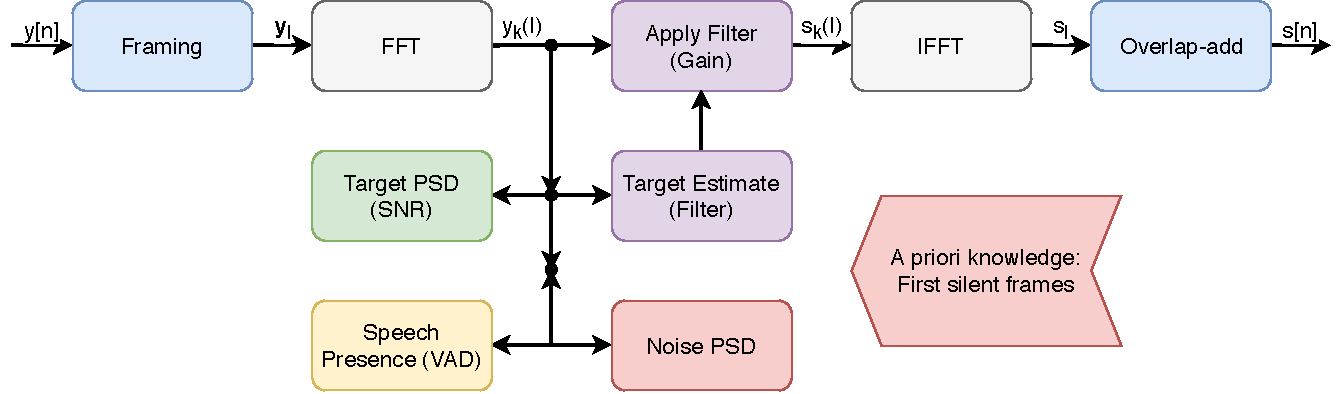
\includegraphics[width=\textwidth]{images/system.pdf}
  \caption{Overview of the system.}
  \label{fig:system}
\end{figure}

This system is focused on a single microphone setup. With a multiple microphone setup, the speech enhancement can be improved upon. Direction estimation and spatial filtering with beamformers can be implemented to filter the unwanted interference and noise from certain directions. This subsystem can be placed before the single microphone speech enhancement system.

The system's functions will be divided into six Sections. The framing and overlap add function will be implemented in Section \ref{sec:framing_overlap_add}. The noise PSD estimation and the source PSD estimation are discussed in Section \ref{sec:noise_estimation} and Section \ref{sec:snr_estimation} respectively. The voice activity detection will be discussed in Section \ref{sec:vad}. With all this information, the target estimation where the filters are designed is discussed in Section \ref{sec:target_estimation}. And lastly, the spatial filtering will be discussed in Section \ref{sec:mm_bf}.

\section{Framing \& Overlap Add} \label{sec:framing_overlap_add}

The first step, as described in Fig. \ref{fig:system}, is the framing of the audio file. This is done according to Eq. \ref{eq:framing}. Where $l$ is the frame index (the l-th frame), $n$ is sample number, $R$ is the hop-length. $w[n]$ is the window used to smoothen the signal in such a way that the signal does not become discontinuous and cause wrong sidelobes when applying the FT.

\begin{equation}
  \label{eq:framing}
  y_{l}[n] = y[n + lR]w[n],\quad n=0,\hdots,N-1
\end{equation}

The last step of the system is the Overlap Add-block. The windowing is removed after which the samples are added back together to one file.
\begin{equation}
  \label{eq:overlap_add}
  y[n] =  \sum_{l=1}^{k} y_{l}[n]/w[n]
\end{equation}

There are various windows that are suited for framing an audio signal. The standard Hamming and Hann window and the square-root Hann window used in a paper by Hendriks\cite{Hendriks} was evaluated. When overlap adding all the frames without applying any changes, the signal should be recovered without any trouble. The overlap added windows should then be equal to an ones vector. Using different values for the overlap percentage, the corresponding overlap add vector is generated and compared to an all-ones vector. An important variable for the framing function is the overlap percentage.  The results in Fig. \ref{fig:opt_oa} show the negative MSE of these two vectors. The peak value is around 70\% for the square-root Hann.

\begin{figure}[h]
  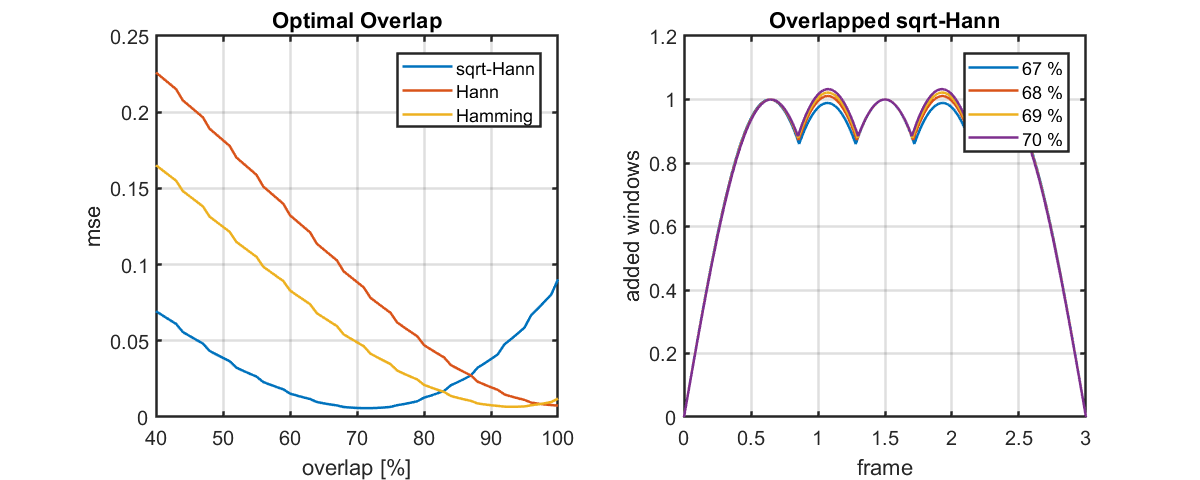
\includegraphics[width=\textwidth]{images/optimal_overlap.png}
  \caption{Optimal overlap percentage for the square-root Hann window.}
  \label{fig:opt_oa}
\end{figure}

\section{Noise PSD Estimation} \label{sec:noise_estimation}
For the noise estimation, it is considered that speech and noise are independent and uncorrelated. From this Eq. \ref{eq:H0} and \ref{eq:H1} can be derived. Whether $H_0$ or $H_1$ corresponds to a particular timeframe is determined by the Voice Activity Detector in Section \ref{sec:vad}.
\begin{align}
  H_{0}: & Y_{K}(l) = N_{k}(l) \quad \text{(speech absence)}
  \label{eq:H0} \\
  H_{1}: & Y_{K}(l) = S_{k}(l) + N_{k}(l) \quad \text{(speech presence)}
  \label{eq:H1}
\end{align}

\subsection{Voice Activity Dectector}
The method used to estimate the noise PSD is based on Voice Activity Detector. This Noise PSD estimation is given as Eq. \ref{eq:smoothingsigma}. Where $\alpha$ is the smoothing constant. As described in \cite{Hendriks}, this method works well for noise with low variation in time.

\begin{equation}
  \sigma_{N,k}^{2}(l)=
  \begin{dcases}
      \alpha \hat \sigma_{N,k}^{2}(l-1) + (1-\alpha)\abs{y_{k}(l)}^{2} & \text{when } H_{0}(l)\\
      \hat \sigma_{N,k}^{2}(l-1) & \text{when } H_{1}(l)
  \end{dcases}
  \label{eq:smoothingsigma}
\end{equation}

In Fig. \ref{fig:VADnoise}, the results are shown. From the figure, the noise is canceled for a great part. Especially in the speech absence regions. This is Because of the Wiener filter, which is discussed in Section \ref{sec:target_estimation}, implementation in combination with the excellent noise estimate when speech is not present. The speech presence regions are uncertain and can have significant errors. This uncertainty is expected to be due to non-optimal variables and reliability on the VAD. When a system becomes more reliable on other system, its robustness could decline when the subsystems are not accurate.

\begin{figure}[h]
  \centering
  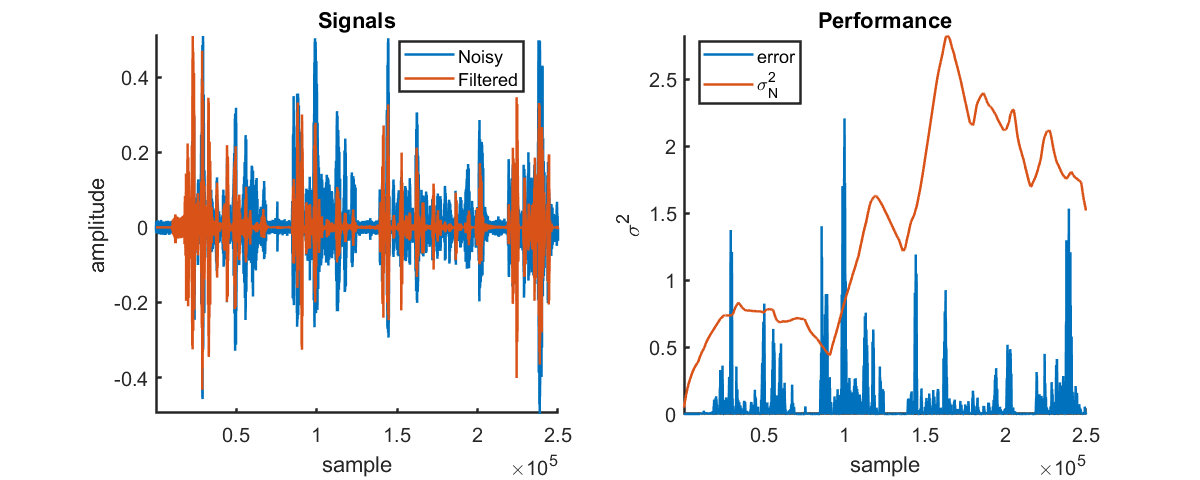
\includegraphics[width=\textwidth]{images/noisepsd.png}
  \caption{Results of the VAD based approach for estimating the noise PSD.}
  \label{fig:VADnoise}
\end{figure}

\clearpage

\subsection{Minimum Statistics Method}
The Minimum Statistics Method does not depend on the Voice Activity Detector and only depends on previous time frames of $y_{k}$ as can be seen in Equation \ref{eq:Q} and \ref{eq:Qmin}. Because using only the minimum value would be a underestimate of $E(|N|^2)$. A biasing factor, $B_{min}$ is added. This biasing factor used is the mean of the 50 previous values of $Q_k(l)$, giving K=50.
\begin{align}
Q_{k}(l) &= \alpha_k(l)Q_k(l-1)+(1-\alpha_k(l))\abs{y_{k}(l)}^{2}\label{eq:Qk} \\
  \mathbf{Q} &=
  \begin{Bmatrix}
    Q_{k}(l-L+1) & \hdots & Q_{k}(l)
  \end{Bmatrix}
  \label{eq:Q} \\
  \hat \sigma_{N,k}^{2}(l) &= B_{min}Q_{min}
  \label{eq:Qmin}\\
\end{align}

In Fig. \ref{fig:minstatnoise}, the results are shown. Here it shows that the noise is canceled very well. When more frames pass, the error increases in voiced areas. This could be due to the bias factor which was added or other mis-estimated variables. It seems to perform better than the VAD based approach in general. A big positive for this method is its independence.

\begin{figure}[h]
  \centering
  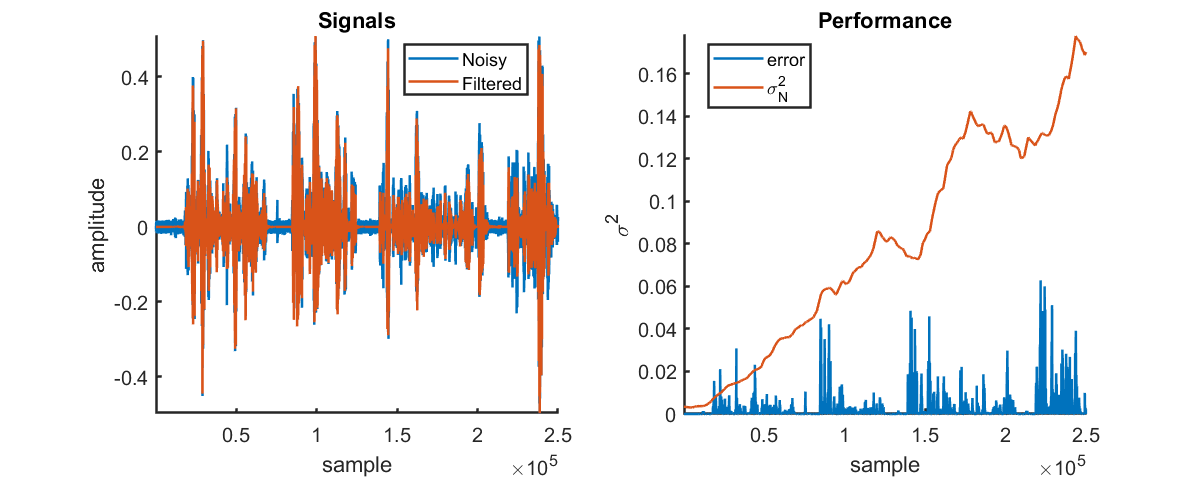
\includegraphics[width=\textwidth]{images/msmethod.png}
  \caption{Results of the Minimal Statistics based approach for estimating the noise PSD (K=50).}
  \label{fig:minstatnoise}
\end{figure}

An important variable is the number of previous frames used. To test the optimal number of previous frames, tests are made for $K=10$ and $K=Inf$. The results of these tests are shown in Fig. \ref{fig:K10} and \ref{fig:KInf}. For a lower amount of previous frames, the error increases. Thus by increasing the amount of previous frames used, the error should decrease. This is shown when all previous frames are used, giving K is infinite. Comparing this to the two tries before indeed shows a lower error present. While compared to K=10, there is a 50\% execution-time increase.
\todo[inline]{K10 en Kinf fixen (onderkant valt er vanaf)}

\begin{figure}[h]
  \centering
  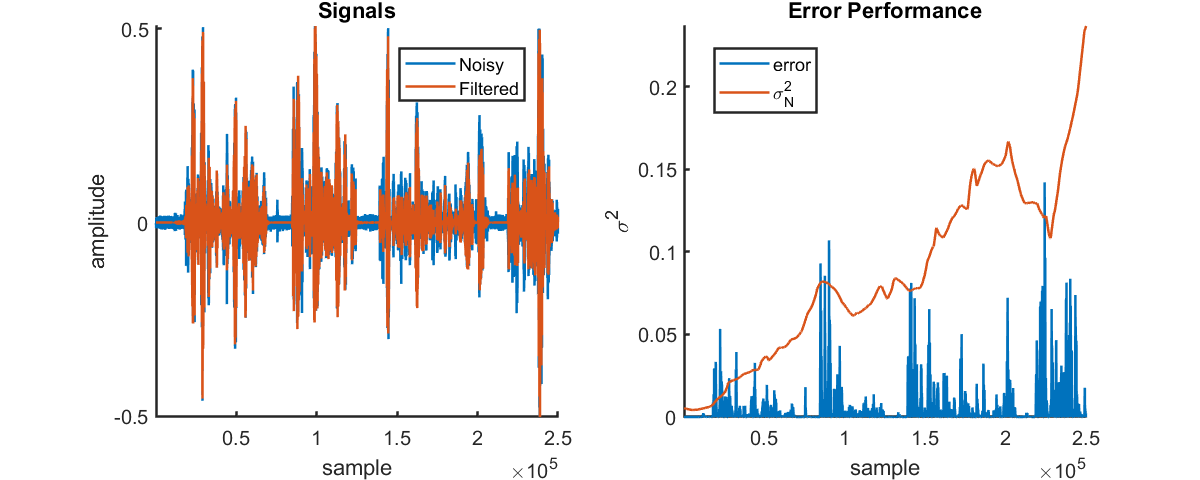
\includegraphics[width=\textwidth]{images/MeanK10.png}
  \caption{Results of the Minimal Statistics based approach using K=10.}
  \label{fig:K10}
\end{figure}

\begin{figure}[h]
  \centering
  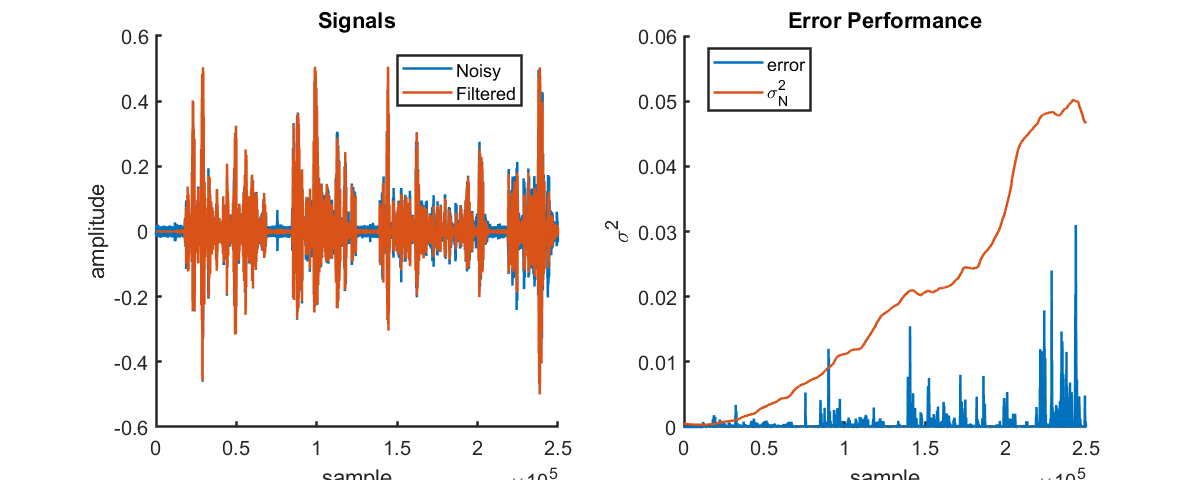
\includegraphics[width=\textwidth]{images/MeanKinf.png}
  \caption{Results of the Minimal Statistics based approach using K=Inf.}
  \label{fig:KInf}
\end{figure}

\clearpage
\subsection{MMSE Method}
One of the more extensive methods discussed during the course is the MMSE Method. Equation \ref{eq:noiseMMSE1} looks similar to Equation \ref{eq:smoothingsigma} when speech is not present. Instead of using the PSD of the input signal $y_k(l)$, the noise its expected value is determined for that specific time-frame. This can be done as in Equation \ref{eq:noiseMMSE2}.
\begin{align}
  \widehat{\sigma_{N}^{2}}(l) &= \alpha \widehat{\sigma_{N}^{2}}(l-1) + (1-\alpha)E\left[ \abs{N_{k}(l)}^{2}\abs{y_{k}(l)}\right]
  \label{eq:noiseMMSE1} \\
  E\left[ \abs{N_{k}(l)}^{2}\abs{y_{k}(l)}\right] &=
  P\left(H_{0,k}(l)|y_{k}(l)\right) E\left[\abs{N_{k}(l)}^{2}\abs{y_{k}(l)},H_{0,k}\right] +
  P\left(H_{1,k}(l)|y_{k}(l)\right) E\left[\abs{N_{k}(l)}^{2}\abs{y_{k}(l)},H_{1,k}\right]
  \label{eq:noiseMMSE2}
\end{align}

There are some unknowns present. The change that speech is absent can be rewritten as in Equation \ref{eq:MMSEu1}. The expected values can be given as Formulas \ref{eq:MMSEu2} and \ref{eq:MMSEu3}.
\begin{align}
  P\left(H_{0,k}(l)|y_{k}(l)\right) &= 1 - P\left(H_{1,k}(l)|y_{k}(l)\right)
  \label{eq:MMSEu1} \\
  E\left[\abs{N_{k}(l)}^{2}\abs{y_{k}(l)},H_{0,k}\right] &= \abs{y_{k}(l)^{2}}
  \label{eq:MMSEu2} \\
  E\left[\abs{N_{k}(l)}^{2}\abs{y_{k}(l)},H_{1,k}\right] &= \widehat{\sigma_{N}^{2}}(l-1)
  \label{eq:MMSEu3}
\end{align}

This leaves only one function to be determined as which can be further broken down as in Equation \ref{eq:MMSEu4}. Of which the two elements are given by Equations \ref{eq:pyh0} and \ref{eq:pyh1}.
\begin{align}
  P\left(H_{1,k}(l)|y_{k}(l)\right) &= \frac{P\left(H_{1,k}(l))\right)p_{Y|H_{1}}}{P\left(H_{1,k}(l))\right)p_{Y|H_{1}} + P\left(H_{0,k}(l))\right)p_{Y|H_{0}}}
  \label{eq:MMSEu4}\\
  p_{Y|H_{0}} &= \frac{1}{\widehat{\sigma_{N}^{2}} \pi} \exp\left(-\frac{\abs{y^{2}}}{\widehat{\sigma_{N}^{2}}}\right)
  \label{eq:pyh0}\\
  p_{Y|H_{0}} &= \frac{1}{\widehat{\sigma_{N}^{2}} (1+\xi_{H_{1}})\pi} \exp\left(-\frac{\abs{y^{2}}}{\widehat{\sigma_{N}^{2}}(1+\xi_{H_{1}})}\right)
  \label{eq:pyh1}
\end{align}

However, $\xi_{H_{1}}$ is unknown and there is no sufficient a priori knowledge present to give an estimation of this variable. Which makes this method unfeasible to use.

\section{SNR Estimation} \label{sec:snr_estimation}

\begin{equation}
  \xi = \frac{\sigma_{S,k}(l)^{2}}{\sigma_{S,k}(l)^{2}} =
  \frac{P_{SS,k}}{P_{NN,k}} =
  \frac{E\left\{\abs{S_{k}(l)}^{2}\right\}}{E\left\{\abs{N_{k}(l)}^{2}\right\}}
  \label{eq:SNR}
\end{equation}

\begin{align}
  \xi_{k}(l) &= \frac{E\left\{\abs{Y_{k}(l)}^{2}\right\}}{E\left\{\abs{N_{k}(l)}^{2}\right\}} - 1
  \label{eq:ML1}\\
  &= \frac{\hat P_{YY,k}^{B}(l)}{\frac{1}{L}E\left\{\abs{N_{k}(l)}^{2}\right\}}
  \label{eq:M2}
\end{align}

\begin{align}
  \xi_{k}(l) &= \alpha \frac{E\left\{\abs{S_{k}(l)}^{2}\right\}}{E\left\{\abs{N_{k}(l)}^{2}\right\}} +
  (1-\alpha)\left(\frac{E\left\{\abs{Y_{k}(l)}^{2}\right\}}{E\left\{\abs{N_{k}(l)}^{2}\right\}} - 1\right)
  \label{eq:dd1}\\
  \abs{S_{k}(l)}^{2} &= \abs{\hat S_{k}(l-1)}^{2}
  \label{eq:dd2} \\
  \frac{E\left\{\abs{Y_{k}(l)}^{2}\right\}}{E\left\{\abs{N_{k}(l)}^{2}\right\}} - 1 &=
  \max \left[(\frac{\abs{Y_{k}(l)}^{2}}{E\left\{\abs{N_{k}(l)}^{2}\right\}}-1,0)\right]
\end{align}

\section{Voice Activity Detection} \label{sec:vad}
For the noise PSD estimation in Section \ref{sec:noise_estimation} and the SNR estimation in Section \ref{sec:snr_estimation}, the pressence of speech is needed to increase the performance of the estimators. The Voice Activity Detector will evaluate the frame and give a speechflag wether speech is present or not.

This can be done by looking at the average energy of the frame. In the case of speech present and a SNR bigger than 0, this should be higher than in the case of noise only. To get a linear scaling with respect to the SNR, the log-energy is calculated. We then can express the energy difference as stated in Eq. \ref{eq:TH0} and Eq. \ref{eq:TH1}. This likelihood function is shown in Eq. \ref{eq:vad1} and Eq. \ref{eq:vad2}.

\begin{align}
  T(l) &= \frac{1}{L} \sum_{k=1}^{k=L} log(\Lambda_{k}(l)) \gtreqless_{H_{0}}^{H_{1}} \lambda
  \label{eq:vad1}\\
  \Lambda_{k}(l) &= P_{YY,k}
  \label{eq:vad2}
\end{align}

\begin{align}
  T(l)_{H_{0}}  &\approx  \sigma_{N}^{2}
  \label{eq:TH0}\\
  T(l)_{H_{1}}  &\approx  \sigma_{N}^{2} + SNR
  \label{eq:TH1}
\end{align}

The threshold for the likelihood function could be a constant which is higher than the noise PSD. When noise is dynamic however, this can not be a constant. A dynamic value can be chosen based on the previous noise estimation and SNR estimation. A value between $\sigma_{N}^{2}$ and $\sigma_{N}^{2} + SNR$ can be chosen.

The results of the VAD can be seen in Fig. \ref{fig:VAD}. These results were made using the Noise and SNR estimates from the previous subsystems.

\begin{figure}[h]
  \centering
  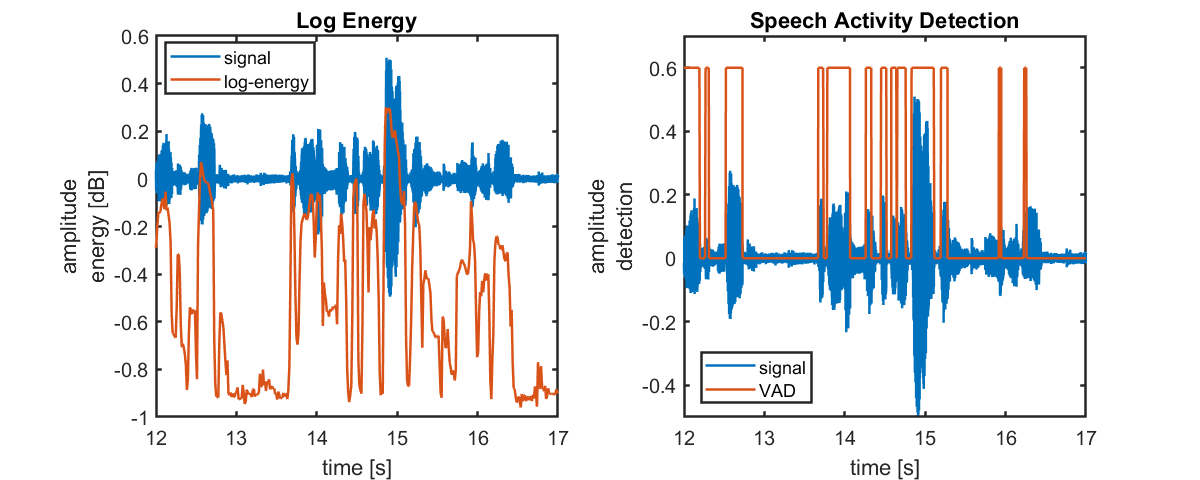
\includegraphics[width=\textwidth]{images/vad.png}
  \caption{Log-energy and VAD performance.}
  \label{fig:VAD}
\end{figure}

\section{Target Estimation} \label{sec:target_estimation}

\begin{align}
  P_{SS,k}(l) &= P_{YY,k}(l) - P_{NN,k}(l)
  \label{eq:psds1} \\
  \widehat{\abs{S_{k}(l)}}^{2} &= \abs{Y_{k}(l)}^{2}-\abs{N_{k}(l)}^{2}
  \label{eq:psds2} \\
  \widehat{\abs{S_{k}(l)}}^{2} &=
  \left(\max{\left\{1-\frac{E\left[\abs{N_{k}(l)}^{2}\right]}{\abs{y_{k}(l)}^{2}},\epsilon\right\}}\right)^{\frac{1}{2}}\abs{y_{k}(l)}
  \label{eq:psds3} \\
  S_{k}(l)^{2} &= \widehat{\abs{S_{k}(l)}}^{2} \dot e^{j\measuredangle y_{k}(l)}
\end{align}

\begin{align}
  \hat{S_{k}} &= H_{k} \dot Y_{k}
  \label{eq:wiener1} \\
  H_{k} &= \frac{P_{SY,k}}{P_{PYY,k}}
  \label{eq:wiener2} \\
  &= \frac{SNR_{k}}{SNR_{k}+1}
  \label{eq:wiener3}
\end{align}

\section{Multi-microphone beamforming} \label{sec:mm_bf}
When using multiple microphones, the spatial properties of the incomming signals can be exploited. Since there is a (small) but relevant  distance difference between the microphones, the time of arrival of the same signal differs. This time delay can be used to estimate the direction of the source and to filter other (interfering) directions.

Before the system is designed and the signals are discussed, some assumptions are made. First of all, the speech and noise are assumed to be  WSS. Secondly a far field is assumed where the angles of arrival at every microphone is identical. These two assumptions can be used to simplify the incoming signals at each microphones. Since the signal is WSS, a time delay can be interpreted as a phase shift in frequency.

Because there is a phase shift, spatial aliasing becomes important. This is where distance between microphones become too big where the periodic signal shifts a full time interval. To avoid this, the distance between microphones should be smaller than half of the wavelength. When assuming a maximum frequency of 8000KHz, the maximum distance between microphones is 2 milimiters.

Since the signal only differs in phase and a linear microphone setup, the signal model for each microphone can be defined as in Eq. \ref{eq:bf}.

\begin{equation}
  \mathbf{Y}_{k}(l) =
  \begin{bmatrix}
    S_{k}(l) & S_{k}(l)e^{-j2\pi\frac{k\tau}{N}} & \hdots & S_{k}(l)e^{-j2\pi(M-1)\frac{k\tau}{N}}
  \end{bmatrix}
  + \mathbf{N}_{k}(l)
  \label{eq:bf}
\end{equation}

In this equation, $\mathbf{Y}_{k}(l)$ can be expressed as a linear combination of $S_{k}(l)$ by a steering vector defined in Eq. \ref{eq:steering}. The resulting model can then be expressed as showed in Eq. \ref{eq:bf_model}.

\begin{equation}
  \mathbf{d}_{k} =
  \begin{bmatrix}
    1 & e^{-j2\pi \frac{k\tau}{N}} & \hdots & e^{-j2\pi(M-1)\frac{k\tau}{N}}
  \end{bmatrix}
  \label{eq:steering}
\end{equation}

\begin{equation}
  \mathbf{Y}_{k}(l) = S_{k}(l)\mathbf{d}_{k} + \mathbf{N}_{k}(l)
  \label{eq:bf_model}
\end{equation}

From this last model, the source signal can easily opbtained by the equation shown in Eq. \ref{eq:bf_sol}. This method is called the delay and sum beamformer, since the first signals are delayed untill all the signals can be added. Results and performance of this beamforer is showed in Fig. \ref{fig:bf}. Where nine microphones were used with a initial SNR of 5 dB and an angle of arival at 90 degrees.

\begin{equation}
   \hat S_{k}(l) =\frac{1}{M} \mathbf{d}_{k}^{H}\mathbf{Y}_{k}(l)
  \label{eq:bf_sol}
\end{equation}

\begin{figure}[h]
  \centering
  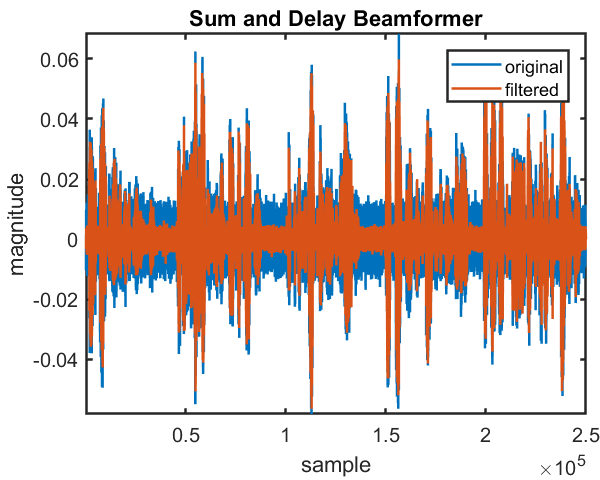
\includegraphics[width=0.5\textwidth]{images/beamformer_sum_delay.png}
  \caption{Performance of the delay and sum beamformer.}
  \label{fig:bf}
\end{figure}

\section{Evaluation and Conclusion} \label{sec:conclusion}
\subsection{Evaluation}
In this Section, more results and evaluation are discussed about the subsystems and the system as a whole.

The most important part of the estimations, is the noise estimation. In Section \ref{sec:noise_estimation}, three methods of noise estimations are discussed where two are implemented. The MMSE estimator was found to need too many prior knowledge. The other methods, the VAD approach and the MS approach have found to be sufficient to reduce the noise in the system. From observations, the VAD approach seemed more unstable. This was due to the debugging and non-optimal fitting of the variables for the VAD and the SNR estimator on which the VAD depended on. The MS approach was found to be more stable and accurate at estimating the noise. This was due to the smoothing and independence.

The SNR estimator was important for the VAD and the Wiener filter. Two methods were implemented. The maximum likelihood approach and the decision directed approach. From observations, the smoothening approach (DD), was found to be more effective at estimating the SNR.

At last, the target estimation is discussed. In Section \ref{sec:target_estimation}, there were two estimators implemented. The Spectral Substraction Method and the Wiener Filter. The Spectral Substraction gave the best absolute error performance and the intelligibility was good. However, some noise remained after filtering. The Wiener filter had a better noise reduction, but succeeded less in keeping the original speech signal. This was found in the absolute error evaluation.

A good evaluation of sources is the Mean Opinion Score, where the result is rated 0 to 5. After rating the result, the mean is taken. This is a preference based evaluation and can vary depending on the evaluating party. For this system, the Spectral Substraction received a MOS value of 1.8 while the Wiener filter received a MOS value of 1.2. This shows that noise reduction is not more important than keeping the voice signal clean.

As a bonus, a beamformer was implemented in Section \ref{sec:mm_bf} to decrease the static noise on the microphones. This was found to be successful depending on the number of microphones. Where more microphones meant a better filtering of the static noise.

\subsection{Conclusion}
From the previous evaluation the conclusion was made that the following subsystems would be used for the single channel noise reduction. For the noise estimation, the Minimum Statistics approach was chosen due to its simplicity and performance when K is large. For the target estimation, the spectral substraction method was chosen due to the MOS rating it received. This means that a VAD and SNR estimation would no longer be needed in the system. From this, we can conclude that the system has a low complexity suited for real time audio processing.


% bibliography
\nocite{*}
\bibliographystyle{IEEEtran}
\bibliography{references}

% appendix is onecolumn
\onecolumn
\appendices \label{sec:appendix}

\section{MATLAB code}
\subsection{Main}
\lstinputlisting{../FinalCodePlekje/main.m}
\clearpage
\subsection{Functions}
\subsubsection{Segment}
\lstinputlisting{../FinalCodePlekje/functions/segment.m}
\subsubsection{vad}
\lstinputlisting{../FinalCodePlekje/functions/vad.m}
\subsubsection{noisePSD}
\lstinputlisting{../FinalCodePlekje/functions/noisePSD.m}
\subsubsection{MinStat}
\lstinputlisting{../FinalCodePlekje/functions/MinStat.m}
\subsubsection{SNR\_ml}
\lstinputlisting{../FinalCodePlekje/functions/snr_ml.m}
\subsubsection{SNR\_dd}
\lstinputlisting{../FinalCodePlekje/functions/snr_dd.m}
\subsubsection{spectral\_substraction}
\lstinputlisting{../FinalCodePlekje/functions/spectral_substraction.m}
\subsubsection{wiener}
\lstinputlisting{../FinalCodePlekje/functions/wiener.m}
\subsubsection{overlap\_add}
\lstinputlisting{../FinalCodePlekje/functions/overlap_add.m}



\end{document}
